\documentclass[11pt,a4paper]{article}

\usepackage[utf8]{inputenc}
\usepackage[hidelinks]{hyperref}
\usepackage{graphicx}
\usepackage{xcolor}
\usepackage{setspace}
\usepackage{amsmath, amssymb}
\usepackage{geometry}
\geometry{margin=1in}

\definecolor{drpblue}{HTML}{0044CC}

\title{\textbf{The Decentralized Rights Protocol (DRP)} \\ 
\large A Blockchain for Human Rights, Proof of Status, and Proof of Activity}
\author{Nkrumah Caleb Joel}
\date{\today}

\begin{document}

\begin{titlepage}
\begin{center}
\vspace{3cm}
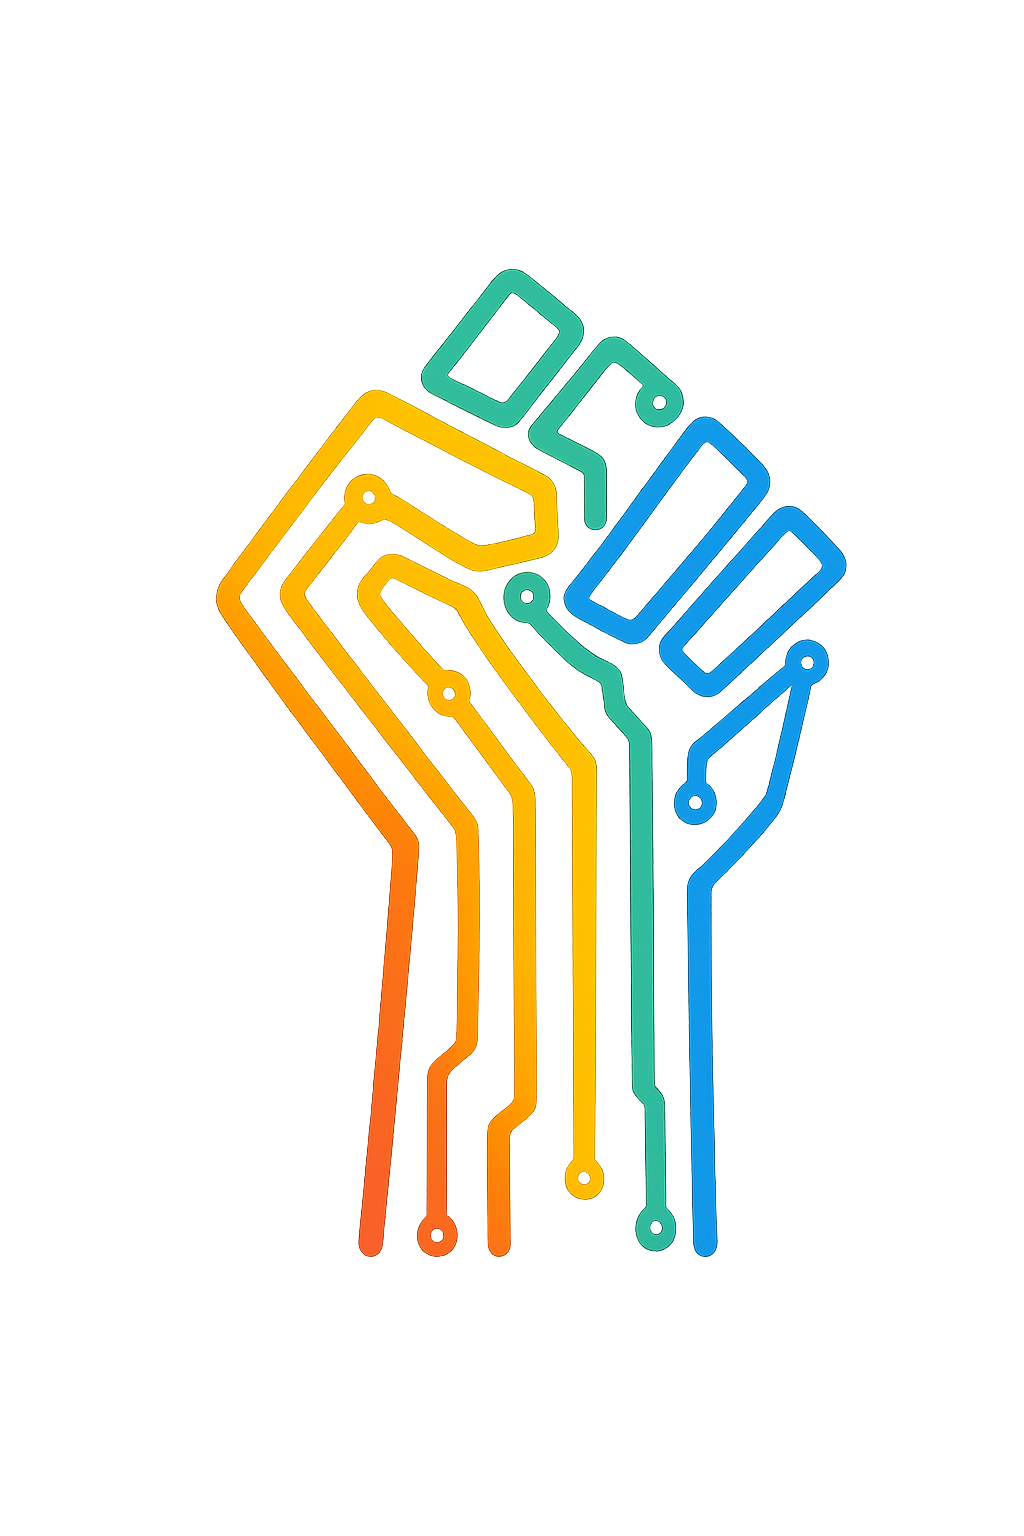
\includegraphics[width=0.3\textwidth]{DRP.png}\\[1cm]
\LARGE\bfseries
\textbf{The Decentralized Rights Protocol (DRP)} \\[0.5cm]
\large A Blockchain for Human Rights, Proof of Status, and Proof of Activity\\[2cm]
\large DRP Research Collective\\[1cm]
\large NeonTechnoX\\[1cm]
\today
\end{center}
\end{titlepage}

\newpage
\tableofcontents
\thispagestyle{empty}

\newpage

% =============================================================================
% SECTION 1: INTRODUCTION
% =============================================================================

\section{Introduction}

The history of blockchain technology has been marked by groundbreaking innovation, but also by structural limitations that prevent it from addressing some of the most pressing challenges of our time. Bitcoin introduced the world to decentralized consensus, demonstrating that value can be transferred without trusted intermediaries. Ethereum expanded this foundation by enabling smart contracts and decentralized applications (dApps), creating programmable trust. However, both approaches, and most successors, have left unresolved issues around fairness, inclusivity, sustainability, and governance.

The Decentralized Rights Protocol (DRP) is conceived as a new paradigm that bridges the gap between digital networks and human rights. Unlike prior systems that primarily measure computational work or economic stake, DRP introduces two novel consensus mechanisms: \textbf{Proof of Status (PoST)} and \textbf{Proof of Activity (PoAT)}. These are not merely technical innovations but moral and societal ones, designed to ensure that blockchain systems contribute to human well-being and equitable global development.

\textbf{Proof of Status} uses artificial intelligence to verify the identity, integrity, and contributions of participants. Rather than rewarding only capital holders, DRP ensures that reputation, verified contributions, and ethical behavior form the basis for influence in the system. This mechanism prevents plutocracy while rewarding authentic participation.

\textbf{Proof of Activity} extends this principle into the real world. Leveraging IoT devices, mobile applications, and secure digital tools, it allows individuals to prove verifiable actions: whether using renewable energy, contributing to education, engaging in civic work, or developing local infrastructure. These activities are cryptographically signed, AI-verified, and sealed into the blockchain, ensuring accountability without compromising privacy.

In addition, DRP introduces the concept of \textbf{AI Elders}, semi-autonomous agents that safeguard consensus. Through quorum-based decision-making, key rotation, and revocation lists, these agents maintain the network's integrity and reduce the risk of centralization. This ensures that DRP operates as a living, evolving system of checks and balances, one that can adapt to new threats and societal needs.

The overarching vision of DRP is not limited to digital finance. It is about embedding fairness, transparency, and human dignity into the very infrastructure of the internet. By aligning blockchain with the principles of human rights, DRP aims to become the foundational protocol for a future where access to food, healthcare, education, and clean water is recognized not as privilege but as entitlement. Its design is guided by global goals, such as the United Nations Sustainable Development Goals (SDGs), while addressing local realities, beginning with pilot deployments in Africa.

This whitepaper outlines the philosophical foundations, technical architecture, governance design, security considerations, and practical implementations of DRP. It also situates DRP within the historical trajectory of blockchain, identifying both the achievements and failures of its predecessors. The reader will find here not just a technical specification, but a roadmap for a more humane and equitable digital future.

% =============================================================================
% SECTION 2: HISTORICAL CONTEXT
% =============================================================================

\section{Historical Context}

\subsection{From Ledgers to Digital Trust}
The history of value exchange has always been bound to the concept of trust. Early societies used clay tablets, shells, and precious metals to record obligations and transfer value. Over time, centralized intermediaries such as banks emerged as custodians of trust, enabling large-scale economic coordination but concentrating power in the hands of a few institutions. This centralization has repeatedly led to crises, from hyperinflation to the collapse of financial systems, and continues to exclude billions of people who remain unbanked.

\subsection{Bitcoin and PoW}
Bitcoin emerged in 2009 as a response to the 2008 financial crisis, introducing the concept of decentralized digital currency through Proof of Work (PoW). While revolutionary in its decentralization, PoW has significant limitations: it consumes enormous amounts of energy, concentrates mining power in regions with cheap electricity, and creates barriers to entry that favor those with capital and technical resources.

\subsection{Ethereum \& Smart Contracts}
Ethereum expanded blockchain's capabilities by introducing smart contracts and decentralized applications. However, its transition from PoW to Proof of Stake (PoS) has created new forms of centralization, where those with more capital have greater influence over network decisions.

\subsection{Governance Experiments (Polkadot, Cardano)}
Polkadot and Cardano have experimented with novel governance models, but they still primarily rely on token ownership for decision-making power, perpetuating plutocratic structures.

\subsection{African Context \& Emergence of DRP}
The African context presents unique challenges and opportunities. From the Organization of African Unity (OAU) to the African Union (AU), there has been a continuous quest for self-determination and equitable development. DRP emerges from this context, designed specifically to address the needs of underserved populations while creating a more inclusive global blockchain ecosystem.

% =============================================================================
% SECTION 3: CORE INNOVATIONS OF DRP
% =============================================================================

\section{Core Innovations of DRP}

\subsection{Proof of Status (PoST)}
Proof of Status represents a paradigm shift from capital-based to contribution-based consensus. It uses AI to verify the identity, integrity, and meaningful contributions of participants. This mechanism ensures that influence in the network is earned through verified actions and ethical behavior rather than simply holding tokens.

\subsection{Proof of Activity (PoAT)}
Proof of Activity extends consensus into the real world by verifying meaningful actions through IoT devices and mobile applications. Participants can prove activities such as using renewable energy, contributing to education, engaging in civic work, or developing infrastructure. These activities are cryptographically signed and AI-verified.

\subsection{AI Elder Agents}
AI Elder Agents are semi-autonomous entities that safeguard network consensus through quorum-based decision-making. They implement key rotation, maintain revocation lists, and ensure network integrity while reducing centralization risks.

\subsection{Dual-Token Economy (\$RIGHTS, \$DeRi)}
DRP implements a dual-token system where \$RIGHTS serves as the governance token and \$DeRi as the utility token. This separation ensures that governance decisions are made by those with verified status and contributions, while utility functions remain accessible to all participants.

\subsection{IoT \& App Ecosystem Integration}
The protocol integrates with IoT devices and mobile applications to capture real-world activities and verify them on-chain. This creates a bridge between digital and physical world contributions.

\subsection{Governance by Contribution}
Unlike traditional blockchain governance that relies on token ownership, DRP implements governance by contribution, where voting power is determined by verified status and meaningful activities rather than capital accumulation.

% =============================================================================
% SECTION 4: TECHNICAL ARCHITECTURE
% =============================================================================

\section{Technical Architecture}

\subsection{Consensus Workflow}
The DRP consensus mechanism combines PoST and PoAT in a hybrid approach. Participants must demonstrate both verified status and ongoing meaningful activities to participate in consensus. The process involves AI verification, cryptographic proofs, and elder quorum validation.

\subsection{Block Structure}
DRP blocks contain traditional transaction data plus status proofs, activity verifications, and elder consensus signatures. The block structure is designed to accommodate the dual consensus mechanisms while maintaining efficiency.

\subsection{Elder Quorum}
The Elder Quorum consists of AI agents that validate consensus decisions. They use threshold signatures and rotation mechanisms to ensure security while preventing centralization.

\subsection{Cryptographic Primitives}
DRP employs advanced cryptographic primitives including zero-knowledge proofs for privacy, threshold signatures for elder consensus, and post-quantum resistant algorithms for future security.

\subsection{Networking Layer}
The networking layer implements efficient gossip protocols for block propagation, activity verification, and elder communication. It's designed for scalability and resilience.

\subsection{Smart Contract Layer}
The smart contract layer supports DRP-specific functions for status verification, activity tracking, and governance operations while maintaining compatibility with existing dApp frameworks.

% =============================================================================
% SECTION 5: CONSENSUS MECHANISM
% =============================================================================

\section{Consensus Mechanism}

\subsection{Overview}
The Decentralized Rights Protocol (DRP) introduces a novel hybrid consensus that combines:
\begin{enumerate}
    \item \textbf{Proof of Status (PoST):} Verification of an individual's identity, contributions, and ethical standing using AI models.
    \item \textbf{Proof of Activity (PoAT):} Verification of real-world or digital activities through IoT devices, trusted applications, and AI agents.
\end{enumerate}

This hybrid consensus ensures that validation power is not merely derived from wealth, but from verified human activity and social contribution.

\subsection{PoST \& PoAT Fusion}
\textbf{Proof of Status (PoST):}
\begin{itemize}
    \item Status is verified by AI agents using identity proofs, contribution records, and social good indicators.
    \item Each participant is assigned a \textbf{Status Score}, a dynamic reputation metric.
    \item Status Scores influence both block validation eligibility and governance voting power.
    \item Mitigates plutocracy by prioritizing verified humans over purely capital-backed validators.
\end{itemize}

\textbf{Proof of Activity (PoAT):}
\begin{itemize}
    \item IoT devices, mobile apps, and tools continuously record verifiable activities.
    \item Activities include renewable energy usage, educational progress, healthcare participation, and digital work contributions.
    \item Activity proofs are aggregated by AI validators to confirm legitimacy.
    \item False or fraudulent activity attempts are flagged by anomaly detection and Elder audits.
\end{itemize}

\subsection{Elder Quorum \& AI Consensus}
AI Elders form a quorum that validates consensus decisions. They use threshold cryptography and rotation mechanisms to ensure security while preventing centralization.

\subsection{Finality \& Fork Resolution}
\textbf{Consensus Flow:}
\begin{enumerate}
    \item Participants broadcast proposed blocks containing both transactions and activity proofs.
    \item AI agents verify activity legitimacy and validate participant status.
    \item Verified blocks are passed to the Elder quorum.
    \item A minimum quorum of Elders co-signs the block for finalization.
    \item Finalized blocks are added to the chain and rewards distributed in \$DeRi tokens.
\end{enumerate}

\textbf{Finality and Fork Resolution:}
\begin{itemize}
    \item \textbf{Finality:} Blocks reach finality once signed by a threshold of Elders and validated by AI.
    \item \textbf{Fork Resolution:} In the event of competing forks, the chain with the highest aggregate \textit{Status + Activity score} is prioritized.
    \item This method prevents traditional 51\% attacks since wealth alone cannot override status/activity legitimacy.
\end{itemize}

\subsection{Energy \& Efficiency}
Unlike PoW systems, DRP is energy-efficient, requiring minimal computational resources for consensus. Energy consumption is focused on meaningful activities rather than arbitrary computation.

\subsection{Security Considerations}
The consensus mechanism is designed to resist various attack vectors including Sybil attacks, nothing-at-stake problems, and long-range attacks through the combination of status verification and activity requirements.

% =============================================================================
% SECTION 6: AI VERIFICATION LAYER
% =============================================================================

\section{AI Verification Layer}

\subsection{AI Models \& Functions}
Artificial Intelligence serves as the verification backbone of the Decentralized Rights Protocol (DRP). Instead of relying solely on human validators or purely deterministic cryptographic proofs, DRP leverages AI to:
\begin{itemize}
    \item Authenticate real-world activities.
    \item Evaluate the legitimacy of participant status.
    \item Detect anomalies, fraud, and collusion attempts.
    \item Provide ethical oversight for sensitive use cases (healthcare, education, human rights).
\end{itemize}

\textbf{AI Models and Functions:}
\begin{enumerate}
    \item \textbf{Identity Verification:} AI models analyze biometric, credential, or behavioral signals to confirm human uniqueness while preserving privacy.
    \item \textbf{Activity Validation:} Computer vision, IoT data ingestion, and NLP pipelines confirm the authenticity of submitted activity proofs.
    \item \textbf{Reputation Scoring:} Machine learning models update dynamic \textbf{Status Scores} based on historical behavior, verified contributions, and social trust.
    \item \textbf{Fraud Detection:} Outlier detection, anomaly clustering, and adversarial resilience mechanisms identify malicious attempts to fake activity.
    \item \textbf{Bias Auditing:} Fairness-aware AI modules ensure that decisions are not skewed by race, gender, geography, or socio-economic conditions.
\end{enumerate}

\subsection{AI Elders \& Quorum}
The verification process integrates human-in-the-loop oversight:
\begin{itemize}
    \item A quorum of \textbf{AI Elders} (specialized agents) co-sign blocks after consensus checks.
    \item Elders rotate periodically via secure key rotation.
    \item An Elder revocation list ensures that compromised or malicious Elders can be revoked without affecting chain stability.
\end{itemize}

\subsection{Transparency \& Accountability}
\begin{itemize}
    \item All AI decisions are accompanied by \textbf{explainability reports}, stored on-chain in hashed form.
    \item Participants may appeal AI-based rejections through Elder arbitration.
    \item Audit logs allow external researchers and governance councils to monitor AI behavior.
\end{itemize}

\subsection{Adversarial Robustness}
\begin{itemize}
    \item AI models are hardened against data poisoning and adversarial attacks.
    \item Secure multi-party computation ensures that AI verifications cannot be manipulated by a single validator.
    \item Federated learning approaches are adopted, so models improve with global data without compromising user privacy.
\end{itemize}

% =============================================================================
% SECTION 7: TOKENOMICS \& ECONOMIC DESIGN
% =============================================================================

\section{Tokenomics \& Economic Design}

\subsection{Dual-Token System (\$RIGHTS \& \$DeRi)}
The DRP ecosystem utilizes a dual-token structure to balance governance, reputation, and economic activity:

\begin{itemize}
    \item \textbf{\$RIGHTS (Governance Token):}
    \begin{itemize}
        \item Represents identity, status, and long-term reputation.
        \item Grants voting power in governance decisions (Elder selection, protocol upgrades).
        \item Staked by Elders to participate in quorum validation.
        \item Non-transferable in some cases to prevent reputation markets.
        \item Distribution: 30\% Community airdrop, 20\% Development team, 25\% DAO Treasury, 15\% Strategic partnerships, 10\% Research grants.
    \end{itemize}

    \item \textbf{\$DeRi (Utility Token):}
    \begin{itemize}
        \item Used for transactions, gas fees, and micro-payments in the DRP-VM.
        \item Distributed as block rewards to activity contributors and validators.
        \item Incentivizes sustainable practices (e.g., renewable energy use, verified educational or health activities).
        \item Can be freely transferred, exchanged, or bridged across chains.
        \item Distribution: 40\% Community rewards, 25\% Elder pool, 15\% Development fund, 10\% Strategic partners, 10\% Reserve.
    \end{itemize}
\end{itemize}

\subsection{Incentives \& Distribution}
The incentive system is designed to reward both verified status and active contributions:

\begin{itemize}
    \item \textbf{Activity Rewards:} IoT devices, apps, or users submitting verified activity logs receive \$DeRi tokens.
    \item \textbf{Status Rewards:} Long-term contributors, educators, and community leaders receive periodic \$RIGHTS allocations.
    \item \textbf{Elder Rewards:} Elders who co-sign blocks earn a combination of \$RIGHTS (status reinforcement) and \$DeRi (transaction fees).
    \item \textbf{Sustainability Rewards:} Verified clean energy usage or eco-friendly activities yield boosted incentives.
\end{itemize}

Token distribution prioritizes verified contributions and meaningful activities rather than capital accumulation, with initial distribution focusing on underserved populations and meaningful contributors.

\subsection{Economic Stability}
The economic model is designed for long-term stability through deflationary mechanisms for \$RIGHTS and inflationary mechanisms for \$DeRi, balanced to maintain purchasing power while encouraging participation.

\subsection{Deflationary/Inflationary Balance}
\begin{itemize}
    \item Transaction fees in \$DeRi are partially burned, reducing inflationary pressure.
    \item \$RIGHTS has a fixed supply and can only be earned through verifiable contributions, not purchased.
    \item Periodic adjustments via governance ensure long-term equilibrium.
    \item \$RIGHTS tokens have a deflationary mechanism to maintain governance value, while \$DeRi tokens have controlled inflation to ensure utility accessibility.
\end{itemize}

\subsection{Sustainability}
The economic model ensures long-term sustainability through activity-based rewards, governance participation incentives, and ecosystem development funding mechanisms.

% =============================================================================
% SECTION 8: GOVERNANCE MODEL
% =============================================================================

\section{Governance Model}

\subsection{Dual-Token Governance}
Governance in the Decentralized Rights Protocol (DRP) is designed to ensure that no single entity or authority can dominate decision-making. Instead, DRP adopts a multi-layered, participatory governance model built upon its native tokens, AI Elders, and community proposals.

\begin{enumerate}
    \item \textbf{\$RIGHTS (Governance Token):} Used for voting, proposal creation, and influencing network direction.
    \item \textbf{\$DeRi (Utility Token):} Used for network fees, staking in verification pools, rewarding activity proofs, and incentivizing sustainable practices.
\end{enumerate}

The governance model balances decentralization, inclusivity, and security while being adaptable to the evolving needs of society.

\subsection{Proposal Lifecycle}
Governance operates through community-driven proposals. The lifecycle is as follows:
\begin{enumerate}
    \item \textbf{Drafting:} Community members submit proposals outlining improvements, new features, or protocol adjustments.
    \item \textbf{Discussion:} Proposals are debated in open forums, with input from both human participants and AI advisors.
    \item \textbf{Elder Review:} AI Elders analyze the proposal for feasibility, ethics, and potential risks, producing an on-chain audit note.
    \item \textbf{Voting:} Token holders cast votes weighted by their stake of \$RIGHTS tokens.
    \item \textbf{Execution:} Proposals that pass quorum and majority thresholds are automatically implemented through smart contract execution.
\end{enumerate}

\subsection{Voting \& Checks and Balances}
\begin{itemize}
    \item \textbf{Quorum Requirements:} A minimum participation threshold ensures proposals are not passed by a minority.
    \item \textbf{AI Oversight:} AI agents flag malicious or unethical proposals before they reach the voting stage.
    \item \textbf{Multi-Elder Co-Signatures:} Governance decisions require approval by an Elder quorum to prevent governance capture.
    \item \textbf{Revocation Powers:} A community-triggered emergency vote can reverse decisions if harmful outcomes are detected.
\end{itemize}

\subsection{Long-Term Evolution}
The governance model is adaptive:
\begin{itemize}
    \item \textbf{Constitutional Upgrades:} Certain rules (e.g., block time, reward schedules, human rights priorities) can only be changed through supermajority votes.
    \item \textbf{Liquid Democracy:} Participants may delegate their voting power to trusted representatives, improving efficiency.
    \item \textbf{Cross-Chain Integration:} Future governance models may synchronize with other blockchains to allow inter-protocol cooperation.
\end{itemize}

% =============================================================================
% SECTION 9: SECURITY \& THREAT MODEL
% =============================================================================

\section{Security \& Threat Model}

\subsection{Threat Landscape}
Security lies at the core of the Decentralized Rights Protocol (DRP). Given that DRP introduces AI-based verification, Proof of Status (PoST), and Proof of Activity (PoAT), the attack surface extends beyond traditional blockchain threats.

\begin{itemize}
    \item \textbf{Network Threats:} DDoS attacks, port scanning, man-in-the-middle interception, and Sybil attacks.
    \item \textbf{Consensus Threats:} Attempts to manipulate Elder quorums, double-signing, or malicious AI-agent coordination.
    \item \textbf{Data Integrity Threats:} Tampering with IoT devices, falsifying activity data, or poisoning AI models.
    \item \textbf{Key Management Risks:} Private key leakage, poor keystore protection, or failure of rotation protocols.
    \item \textbf{Application Threats:} Smart contract exploits, injection vulnerabilities, or API endpoint exposure.
\end{itemize}

\textbf{Adversary Models:}
\begin{enumerate}
    \item \textbf{External Attackers:} Hackers seeking financial gain, disruption, or reputation damage.
    \item \textbf{Malicious Validators:} Rogue Elders attempting quorum collusion.
    \item \textbf{Data Manipulators:} Adversaries submitting falsified Proof of Activity via compromised IoT devices.
    \item \textbf{State-Level Actors:} Governments or corporations attempting censorship or large-scale disruption.
\end{enumerate}

\subsection{Consensus \& Application Security}
DRP adheres to a multi-layered "defense-in-depth" model:

\textbf{Security Principles:}
\begin{itemize}
    \item \textbf{Minimal Attack Surface:} Only required ports are open; APIs are protected via rate-limiting and strong authentication.
    \item \textbf{Encryption Everywhere:} TLS for all connections; data at rest secured with AES-256; communication signed with ECDSA.
    \item \textbf{Zero Trust Architecture:} Every device, user, and AI agent is verified continuously through PoST and PoAT.
    \item \textbf{Auditability:} All AI and Elder decisions are logged and cross-verified by multiple quorum members.
\end{itemize}

\textbf{Key Management:}
\begin{itemize}
    \item Use of \textbf{Hardware Security Modules (HSMs)} or secure enclaves to store private keys.
    \item Regular \textbf{key rotation} with automated expiration policies.
    \item \textbf{Elder Revocation Lists (ERLs)} to expel compromised validators quickly.
    \item Prohibition against storing private keys (.keystore) in public repositories.
\end{itemize}

\textbf{Consensus Security:}
\begin{itemize}
    \item Elder quorums require multi-signature approvals.
    \item Randomized selection of Elder subsets to reduce collusion risk.
    \item AI-agents apply anomaly detection to spot irregular validation behavior.
\end{itemize}

\textbf{Application Security:}
\begin{itemize}
    \item Continuous penetration testing and bug bounties.
    \item Formal verification of smart contracts where possible.
    \item Protection against replay attacks via nonce-based transaction schemes.
\end{itemize}

\subsection{Incident Response}
\begin{enumerate}
    \item Rapid detection through AI-driven monitoring of network traffic and activity submissions.
    \item Automatic quarantine of compromised nodes or devices.
    \item Transparent disclosure to the community via on-chain governance logs.
\end{enumerate}

\subsection{Post-Quantum Security}
DRP is designed with post-quantum security in mind, implementing quantum-resistant cryptographic algorithms and preparing for future quantum computing threats.

\subsection{Ethical Safeguards}
The system includes ethical safeguards to prevent misuse, ensure privacy protection, and maintain alignment with human rights principles. This includes AI ethics committees and regular audits.

% =============================================================================
% SECTION 10: CASE STUDIES \& APPLICATIONS
% =============================================================================

\section{Case Studies \& Applications}

\subsection{Healthcare Access}
\begin{itemize}
    \item \textbf{Problem:} Millions lack access to healthcare due to inequitable distribution and corruption.
    \item \textbf{DRP Solution:} Proof of Status (PoST) can verify a patient's eligibility for basic healthcare entitlements. Proof of Activity (PoAT) ensures doctors, clinics, and community health workers are active and legitimate.
    \item \textbf{Outcome:} Improved transparency in health resource distribution, fraud prevention in medical aid programs, and equitable access to treatment.
    \item AI-verified patient activity ensures fair distribution of medical resources.
    \item Blockchain-based medical records prevent tampering and provide privacy-preserving portability.
    \item Smart contracts allocate medication, healthcare credits, or doctor consultations based on verified need.
\end{itemize}

\subsection{Education \& Skills Verification}
\begin{itemize}
    \item \textbf{Problem:} Academic fraud and lack of trust in digital learning credentials.
    \item \textbf{DRP Solution:} PoST can confirm a student's enrollment and participation. PoAT validates learning activities (assignments, projects, attendance) via IoT and AI tracking.
    \item \textbf{Outcome:} Authentic educational records, AI-signed digital certificates, and democratized access to learning resources.
    \item Verified learning proofs (attendance, participation, assignments) recorded on-chain.
    \item AI quizzes tied to Proof of Activity ensure students gain knowledge before resource allocation.
    \item Cross-border recognition of qualifications via blockchain credentials.
    \item Educational funding and scholarships allocated based on transparent status verification.
\end{itemize}

\subsection{Food Security \& Agriculture}
\begin{itemize}
    \item \textbf{Problem:} Farmers lack proof of their production activities, making them ineligible for subsidies or fair pricing.
    \item \textbf{DRP Solution:} IoT sensors and drones provide data for PoAT, verifying cultivation, irrigation, and harvests. PoST ensures that legitimate farmers gain access to markets and credits.
    \item \textbf{Outcome:} Reduced fraud in agricultural subsidies, better crop traceability, and fairer access to global supply chains.
    \item Proof of Activity tokens can verify farming work and supply chain transparency.
    \item Food vouchers distributed on-chain, redeemable through verified activity and need.
    \item Prevention of fraud in aid distribution using Elder quorum verification.
\end{itemize}

\subsection{Energy \& Sustainability}
\begin{itemize}
    \item \textbf{Problem:} Greenwashing and unverifiable claims of renewable energy use.
    \item \textbf{DRP Solution:} IoT devices (smart meters, solar panels, wind sensors) feed into PoAT to verify actual clean energy generation and consumption. PoST rewards households or organizations meeting sustainability thresholds.
    \item \textbf{Outcome:} Transparent green credits, incentives for renewable adoption, and measurable contributions toward UN SDGs.
    \item Users rewarded for adopting renewable energy sources (solar, wind, hydrogen fuel cells).
    \item AI-driven Proof of Activity encourages eco-friendly practices (waste recycling, energy saving).
    \item Carbon footprint tracking and offsets secured on-chain.
\end{itemize}

\subsection{Governance \& Social Justice}
\begin{itemize}
    \item \textbf{Problem:} Weak institutions, corruption, and lack of trust in governance.
    \item \textbf{DRP Solution:} PoST can verify identity and citizenship status without exposing personal data. PoAT validates civic activities such as voting, volunteering, or community service.
    \item \textbf{Outcome:} Transparent governance, immutable evidence in social justice cases, and accountability for elected representatives.
    \item Anonymous reporting of crimes, harassment, or violations immutably logged.
    \item AI Elders provide unbiased evidence verification in sensitive cases.
    \item Blockchain voting ensures transparent and tamper-proof democratic processes.
    \item Decentralized dispute resolution with Elder quorum oversight.
\end{itemize}

\subsection{Humanitarian Aid (Pilot in Ghana)}
\begin{itemize}
    \item \textbf{Problem:} Corruption, fraud, and inefficiency in aid delivery.
    \item \textbf{DRP Solution:} PoST verifies beneficiary eligibility. PoAT validates NGO and volunteer activity, ensuring aid is distributed fairly and actively tracked.
    \item \textbf{Outcome:} Reduced diversion of aid, real-time monitoring of distribution, and trust restoration in humanitarian efforts.
    \item \textbf{Background:} Ghana serves as an initial testbed for DRP's Proof of Status and Proof of Activity.
    \item \textbf{Implementation:} IoT devices verify renewable energy usage in rural communities, while PoST ensures that healthcare entitlements are distributed fairly.
    \item \textbf{Impact:} Early simulations demonstrate improved trust in aid distribution and sustainable development efforts.
\end{itemize}

\subsection{Project Lazarus (Asset Recovery)}
Project Lazarus showcases DRP's ability to recover and redistribute lost or stolen assets through ethical and transparent processes.

% =============================================================================
% SECTION 11: IMPLEMENTATION ROADMAP
% =============================================================================

\section{Implementation Roadmap}

\subsection{Phase I: Research \& Design}
The initial phase focuses on foundational research, design, and small-scale testing:
\begin{itemize}
    \item Literature review of blockchain consensus, AI verification systems, and IoT integration.
    \item Development of prototype Proof of Status and Proof of Activity algorithms.
    \item Security research on cryptographic primitives, quantum resistance, and Elder key management.
    \item Simulation of consensus under various network conditions.
\end{itemize}

\subsection{Phase II: Prototype \& Testnet}
The DRP Testnet will serve as an experimental environment for developers, validators, and researchers:
\begin{itemize}
    \item Deployment of a functional blockchain with PoST/PoAT modules.
    \item Elder AI Agents integrated into verification workflows.
    \item IoT and mobile device activity verification proof-of-concept.
    \item Bug bounty program and external security audits.
\end{itemize}

\subsection{Phase III: Mainnet Launch \& Airdrop}
The mainnet rollout establishes DRP as a live, global blockchain protocol:
\begin{itemize}
    \item Genesis block creation with AI-signed Proof of Status.
    \item Decentralized Elder quorum operational at global scale.
    \item Initial distribution of \$RIGHTS governance tokens and \$DeRi utility tokens.
    \item Integration with wallets, exchanges, and dApp ecosystems.
\end{itemize}

\subsection{Phase IV: Governance Growth}
Following mainnet stability, governance and ecosystem expansion begin:
\begin{itemize}
    \item Activation of on-chain governance powered by \$RIGHTS.
    \item Expansion of Project Lazarus for ethical asset recovery.
    \item Establishment of DRP research consortiums across academia, industry, and humanitarian groups.
    \item Grants program to incentivize development of DRP-based applications.
\end{itemize}

\subsection{Phase V: Scaling \& Global Adoption}
The long-term phase focuses on scaling, interoperability, and adoption:
\begin{itemize}
    \item Cross-chain bridges for interoperability with Ethereum, Polkadot, Bitcoin, and other networks.
    \item Full integration with IoT and edge computing devices for real-time Proof of Activity.
    \item AI-augmented consensus optimization for faster throughput.
    \item Deployment in developing regions to achieve UN SDG targets (healthcare, education, food security).
\end{itemize}

\textbf{Milestones:}
\begin{itemize}
    \item \textbf{Year 1:} Testnet deployment, bug bounty, initial governance model.
    \item \textbf{Year 2:} Mainnet launch, token distribution, Elder quorum establishment.
    \item \textbf{Year 3:} Project Lazarus release, ecosystem growth, cross-chain interoperability.
    \item \textbf{Year 5:} Full IoT integration, global adoption in humanitarian applications.
\end{itemize}

% =============================================================================
% SECTION 12: MATHEMATICAL FOUNDATIONS
% =============================================================================

\section{Mathematical Foundations}

\subsection{Notation}
Mathematical notation and definitions used throughout the protocol specification:
\begin{itemize}
    \item $PoST_i$: Proof of Status for participant $i$
    \item $PoAT_i$: Proof of Activity for participant $i$
    \item $S_i$: Status Score for participant $i$
    \item $A_i$: Activity Score for participant $i$
    \item $E_j$: Elder agent $j$
    \item $Q$: Elder Quorum threshold
    \item $\tau$: Consensus threshold
\end{itemize}

\subsection{Consensus Equations (PoST/PoAT)}
Mathematical formulation of the consensus mechanisms:

\textbf{Status Score Calculation:}
$$S_i = \alpha \cdot I_i + \beta \cdot C_i + \gamma \cdot R_i$$

where:
\begin{itemize}
    \item $I_i$: Identity verification score
    \item $C_i$: Contribution score
    \item $R_i$: Reputation score
    \item $\alpha, \beta, \gamma$: Weighting factors
\end{itemize}

\textbf{Activity Score Calculation:}
$$A_i = \sum_{k=1}^{n} w_k \cdot a_{i,k}$$

where:
\begin{itemize}
    \item $a_{i,k}$: Activity $k$ for participant $i$
    \item $w_k$: Weight for activity type $k$
    \item $n$: Total number of activity types
\end{itemize}

\textbf{Consensus Eligibility:}
$$\text{Consensus\_Eligible}_i = \begin{cases} 
1 & \text{if } S_i \geq \tau_S \text{ and } A_i \geq \tau_A \\
0 & \text{otherwise}
\end{cases}$$

\subsection{Reward Functions \& Token Emission}
Mathematical models for token rewards and emission schedules:

\textbf{Block Reward Distribution:}
$$R_{block} = R_{base} \cdot (1 + \lambda \cdot A_{avg})$$

where:
\begin{itemize}
    \item $R_{base}$: Base block reward
    \item $\lambda$: Activity multiplier factor
    \item $A_{avg}$: Average activity score in the block
\end{itemize}

\textbf{Individual Reward:}
$$R_i = \frac{S_i \cdot A_i}{\sum_{j=1}^{n} S_j \cdot A_j} \cdot R_{block}$$

\textbf{Token Emission Schedule:}
$$E(t) = E_0 \cdot e^{-\delta t}$$

where:
\begin{itemize}
    \item $E_0$: Initial emission rate
    \item $\delta$: Decay rate
    \item $t$: Time period
\end{itemize}

\subsection{Game-Theoretic Analysis}
Game-theoretic analysis of the protocol's incentive mechanisms and security properties.

\subsection{Stability \& Convergence of AI Elders}
Mathematical analysis of AI Elder convergence, stability properties, and consensus guarantees.

% =============================================================================
% SECTION 13: CONCLUSION
% =============================================================================

\section{Conclusion}

The Decentralized Rights Protocol represents a fundamental shift in blockchain design, moving from capital-based to contribution-based consensus. By integrating Proof of Status and Proof of Activity with AI Elder governance, DRP creates a system that rewards meaningful contributions while ensuring security and decentralization.

The protocol's dual-token economy, comprehensive security model, and focus on real-world applications position it as a foundational infrastructure for human rights and equitable development. Through pilot programs and gradual scaling, DRP aims to demonstrate that blockchain technology can serve humanity's highest aspirations.

The mathematical foundations, security analysis, and implementation roadmap provide a clear path forward for realizing this vision. As the protocol evolves, it will continue to adapt to new challenges while maintaining its core principles of fairness, transparency, and human dignity.

Key achievements of DRP include:
\begin{itemize}
    \item \textbf{Democratized Consensus:} Moving beyond wealth-based validation to contribution-based participation
    \item \textbf{AI-Enhanced Security:} Leveraging artificial intelligence for robust verification and fraud detection
    \item \textbf{Real-World Impact:} Connecting blockchain technology to meaningful human activities and social good
    \item \textbf{Sustainable Design:} Energy-efficient consensus that rewards environmental responsibility
    \item \textbf{Global Accessibility:} Designed specifically to address the needs of underserved populations
\end{itemize}

The future of DRP lies in its ability to scale these innovations globally while maintaining the core values that make it unique. Through continued research, development, and community engagement, DRP will evolve into a comprehensive platform for human rights, social justice, and equitable development.

% =============================================================================
% SECTION 14: REFERENCES
% =============================================================================

\section{References}

\begin{thebibliography}{99}

\bibitem{nakamoto2008bitcoin}
Nakamoto, Satoshi.
\textit{Bitcoin: A Peer-to-Peer Electronic Cash System}.
2008.

\bibitem{wood2014ethereum}
Wood, Gavin.
\textit{Ethereum: A Secure Decentralised Generalised Transaction Ledger}.
Ethereum Project Yellow Paper, 2014.

\bibitem{un2015sdgs}
United Nations.
\textit{Transforming our world: the 2030 Agenda for Sustainable Development}.
Resolution adopted by the General Assembly, 2015.

\bibitem{oau1963charter}
Organization of African Unity.
\textit{Charter of the Organization of African Unity}.
1963.

\bibitem{au2000constitutive}
African Union.
\textit{Constitutive Act of the African Union}.
2000.

\bibitem{buterin2017governance}
Buterin, Vitalik.
\textit{Notes on Blockchain Governance}.
Vitalik.ca, 2017.

\bibitem{polkadot2017whitepaper}
Wood, Gavin.
\textit{Polkadot: Vision for a Heterogeneous Multi-Chain Framework}.
Web3 Foundation, 2017.

\bibitem{cardano2017whitepaper}
Hoskinson, Charles.
\textit{Cardano: A Decentralized Public Blockchain and Cryptocurrency Project}.
Input Output Hong Kong, 2017.

\bibitem{goodfellow2016deep}
Goodfellow, Ian, et al.
\textit{Deep Learning}.
MIT Press, 2016.

\bibitem{shamir1979share}
Shamir, Adi.
\textit{How to share a secret}.
Communications of the ACM, 1979.

\bibitem{bellare1997hash}
Bellare, Mihir, and Phillip Rogaway.
\textit{The exact security of digital signatures—how to sign with RSA and Rabin}.
Advances in Cryptology—EUROCRYPT'96, 1997.

\bibitem{merkle1988digital}
Merkle, Ralph C.
\textit{A digital signature based on a conventional encryption function}.
Conference on the Theory and Application of Cryptographic Techniques, 1988.

\end{thebibliography}

\end{document}
